\chapter{Die Beschleunigeranlage FAIR unter besonderer Betrachtung des \pnd{}-Detektors}

Da der Track-Cleaner in Zusammenhang mit dem \pnd{}-Experiment entwickelt wurde, soll nun auf das zugrunde liegende physikalische Experiment eingegangen werden. Dazu wird zunächst die Beschleunigeranlage FAIR erklärt, um dann im weiteren Verlauf des Kapitels den \pnd{}-Detektor zu erläutern. Da der \pnd{}-Detektor aus mehreren Subdetektoren besteht, wird im Folgenden die Funktionsweise des Straw Tube Trackers (STT) thematisiert. In diesem Zusammenhang wird auf die Problematik des Trackfindings eingegangen, um somit die Entwicklung eines Track-Cleaners zu motivieren.

\section{FAIR - Facility for Antiproton and Ion Research}
\begin{figure}
  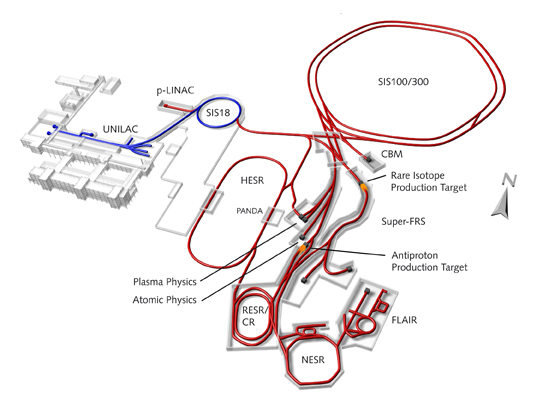
\includegraphics[width=0.7\textwidth]{Bilder/Fair}
	\label{fig:FAIR}
	\caption{Schematische Darstellung der Beschleunigeranlage FAIR}
\end{figure}

Eine schematische Darstellung von FAIR findet sich in Abbildung \ref{fig:FAIR}. Die bereits bestehenden Komponenten der Gesellschaft für Schwerionenforschung sind in blau dargestellt und werden in FAIR integriert. Diese sind in der Abbildung mit SIS18 bezeichnet und werden in Zukunft als Vorbeschleuniger für Protonen benutzt. Diese werden danach in den Doppelring (SIS100) eingespeist und auf bis zu 29GeV beschleunigt. GeV steht für die kinetische Energie in Giga-Elektronvolt. Die Beschleunigung eines Protons auf 29GeV entspricht einer Geschwindigkeit von $2.9\cdot10^8\frac{m}{s}$ bzw. dem 0.9995-fachen der Lichtgeschwindigkeit. Da in FAIR mehrere Experimente zusammengefasst werden sollen, schließen sich danach mehrere Möglichkeiten der Strahlführung an, um den Teilchenstrahl auf die verschiedenen Experimente zu verteilen. Für das \pnd{}-Experiment wird der Strahl zunächst auf ein Wolfram-Target geschossen, um die für \pnd{} benötigten Antiprotonen zu erzeugen. Diese werden dann im Collector Ring (CR) gesammelt, gekühlt und in den High-Energy Storage Ring (HESR) eingespeist. Dort werden die Antiprotonen zunächst auf 14.5 GeV beschleunigt und dann in das am HESR platzierte \pnd{}-Experiment eingeführt. Darauf wird nun im Folgenden genauer eingegangen. \cite[S. 5]{MasterJette}



\section{\pnd{} - Antiproton ANnhilation at DArmstadt}
\label{sec:Panda}
Um die Funktionsweise des Trackfindings zu verstehen, wird nun zunächst der \pnd{}-Detektor erklärt. Dazu wird zuerst auf die physikalische Bedeutung von \pnd{} eingegangen und später der Aufbau des Detektors erläutert.

\subsection{Physikalische Bedeutung von \pnd{}}
\pnd{} beschäftigt sich mit der starken Kraft und den damit zusammenhängenden Wechselwirkungen. Die starke Kraft ist dafür verantwortlich, dass die Nukleonen eines Atomkerns zusammengehalten werden. Durch Experimente mit hochenergetischen Antiprotonenstrahlen soll in \pnd{} die starke Kraft untersucht werden. Dabei werden Antiproton-Proton-Annihilationen und die Reaktionen von Antiprotonen mit schweren Kernen betrachtet. Annihilation beschreibt den Prozess der Paarvernichtung eines Fundamentalteilchens, welches mit seinem korrespondierenden Antiteilchen zusammenstößt. 
\cite[S. 5]{MasterJette} 

\pnd{} wurde so konstruiert, dass verschiedene Experimente mit dem selben Detektorsystem durchgeführt werden können. Diese Experimente lassen sich wie folgt klassifizieren \cite{PANDA_physics_overview}:

\label{panda_experimentklassen}
\begin{description}
	\item[Hadronenspektroskopie] Dieses Aufgabenfeld beschäftigt sich mit der Suche nach exotischen Anregungszuständen von Hadronen. Damit soll die starke Wechselwirkung genauer untersucht werden.
	\item[Nukleonenstruktur] Hier soll der innere Aufbau von Nukleonen genauer erforscht werden, um Rückschlüsse auf Struktur und Bestandteile von Atomkernen ziehen zu können.
	\item[Hadronen in Materie] Um den Ursprung der Hadronenmasse zu verstehen, sollen Hadronen in einem Nuklearen Medium untersucht werden.
	\item[Hyperkerne] Wird bei einem Nukleon ein up- oder ein down-Quark durch ein Strange-Quark ersetzt entstehen Hyperkerne. Durch die Einführung der Strangeness entsteht ein weiterer Freiheitsgrad und somit eine weitere Achse im Nuklear-Diagramm. Diese neuartigen Elemente sollen genauer untersucht werden.
\end{description}

\subsection{Aufbau des Detektors}
\begin{figure}
  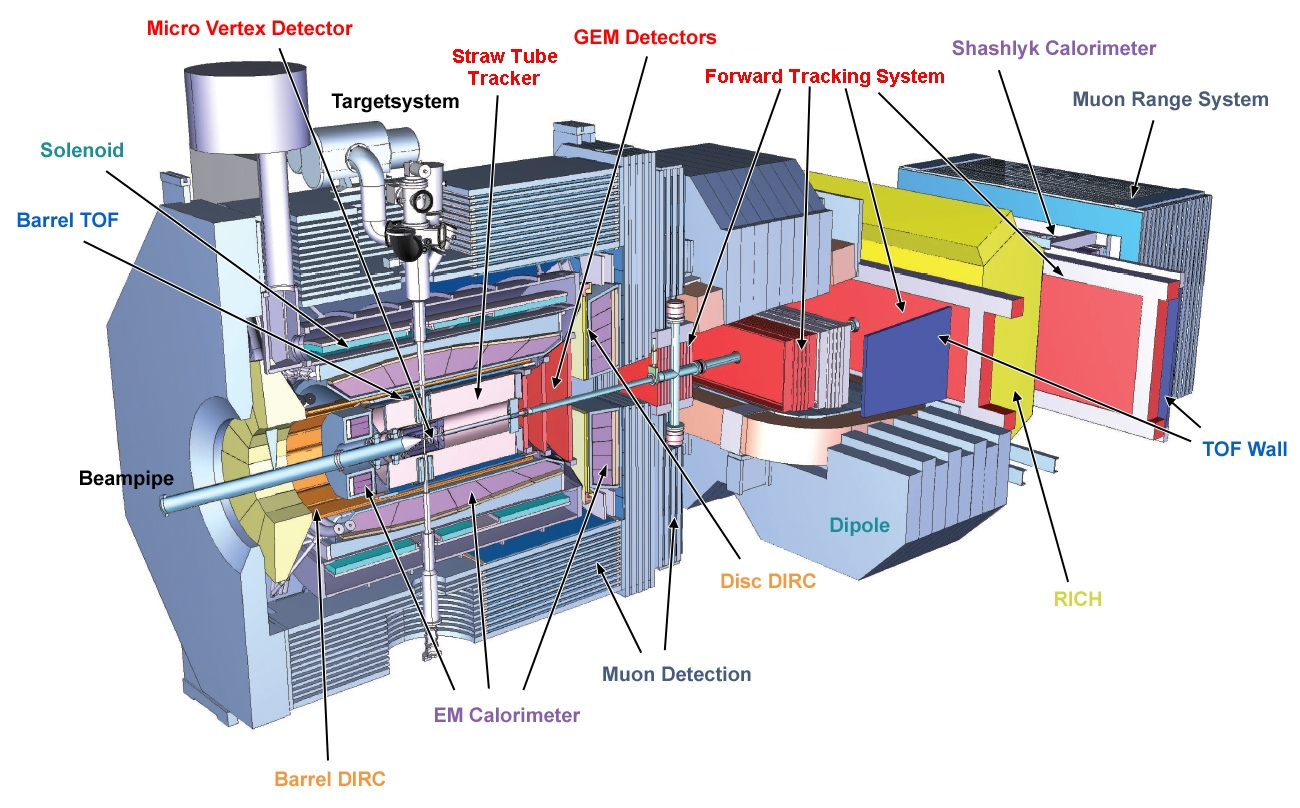
\includegraphics[width=0.9\textwidth]{Bilder/panda_full_detektor}
	\label{fig:panda_full}
	\caption{Schematische Darstellung des gesamten \pnd{}-Detektors}
\end{figure}
Bei dem \pnd{}-Detektor handelt es sich um ein komplexes Detektorsystem, welches aus vielen verschiedenen Subdetektoren zusammengesetzt ist. Eine schematische Darstellung des gesamten \pnd{}-Detektors findet sich in Abbildung \ref{fig:panda_full}. Über das Strahlrohr gelangt der Antiprotonenstrahl zum zentral platzierten Targetsystem. Das Targetsystem ist austauschbar, sodass es an die in Abschnitt \ref{panda_experimentklassen} erwähnten Experimenttypen angepasst werden kann. Das Targetmaterial lässt sich über das Targetsystem zum Stoßpunkt befördern, wo es dann mit dem Antiprotonenstrahl kollidiert. Dabei entsteht eine große Anzahl an Sekundärteilchen, welche sich vom Stoßpunkt aus in verschiedene Richtungen bewegen. Um aus dem Experiment physikalisch wertvolle Ergebnisse folgern zu können, müssen die entstandenen Teilchen möglichst genau rekonstruiert werden. Dazu befindet sich eine Vielzahl unterschiedlicher Detektoren um den Stoßpunkt herum. Diese lassen sich aufgrund ihrer Aufgabe kategorisieren. Der Micro-Vertex-Detektor (MVD), der Straw Tube Tracker/Central Tracker (STT), der Gas Electron Multiplier Detector (GEM), und das Forward Tracking System (FTS) sind spurgebende Detektoren, welche versuchen die Teilchenflugbahn zu rekonstruieren. Darüber hinaus gibt es die Detektoren Detection of Internally Reflected Cherenkov Light (DIRC), Time of Flight System (TOF) und Aerogel Ring Imaging Cherenkov Counter (RICH), welche zur Teilchenidentifikation dienen. Zur Impulsbestimmung befindet sich sowohl im vorderen, als auch im hinteren Teil des \pnd{}-Detektors ein Magnetspektrometer . Das Target-Spektrometer mit einem 2T Solenoid Magnetfeld befindet sich beim Stoßpunkt. Beim Forward-Spektrometer handelt es sich um ein 2Tm Dipol-Magnetfeld, welches sich im hinteren des Detektors befindet. Somit lässt sich der Detektor als Ganzes in zwei Teile aufteilen. Mit dem Target-Spektrometer werden die Teilchen erfasst, deren Flugbahn einen vergleichsweise hohen Polarwinkel aufweisen. Das Forward-Spektrometer erfasst die Teilchen, welche sich im Wesentlichen in Richtung des Antiprotonenstrahls bewegen. Die Funktionsweise der Magnetspektrometern macht sich die Eigenschaften der Lorentzkraft zu Nutze. Ein geladenes Teilchen erfährt beim Durchqueren eines Magnetfeldes $B$ die Kraft $\vec{F_L}=q(\vec{v} \times \vec{B})$, wobei $\vec{v}$ die Bewegungsrichtung, $\vec{B}$ die magnetische Flussdichte und $q$ die Ladung ist. Bei Kenntnis von Teilchenflugbahn und Magnetfeldstärke lassen sich also Rückschlüsse auf die Ladung des Teilchens $q$ ziehen. Die Magneten selber erzeugen dabei keine Messwerte, sondern verursachen nur das zur Ablenkung des Teilchens benötigte Magnetfeld. \cite{PANDA_detektor} \cite[S. 7-10]{MasterJette}
Aufgrund der ablenkenden Wirkung des Magnetfeldes ergeben sich im Target-Spektrometer im Idealfall helixförmige Flugbahnen. Es kann jedoch zu Wechselwirkungen mit dem Detektormaterial kommen, was zum Energieverlust der Teilchen führt. In diesem Fall reduziert sich der Radius der Kreisbewegung mit fortschreitendem Energieverlust.
\cite[S. 11]{MasterJette}

\section{STT - Straw Tube Tracker}
\begin{figure}
  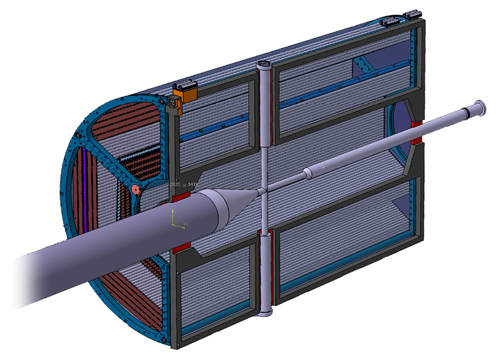
\includegraphics[width=0.9\textwidth]{Bilder/panda_stt}
	\label{fig:panda_stt}
	\caption{Schematische Darstellung des Straw Tube Trackers}
\end{figure}
Im Folgenden wird nun der Straw Tube Tracker genauer betrachtet. Beim STT handelt es sich, wie im vorangegangenen Abschnitt erläutert, um einen spurgebenden Detektor, dessen Aufgabe es ist Teilchenflugbahnen zu rekonstruieren. Wie in Abbildung \ref{fig:panda_stt} ersichtlich, umschließt der STT den Stoßpunkt. Die Aufgabe des STTs besteht darin, die spiralförmigen Flugbahnen von geladenen Teilchen mit möglichst hoher Auflösung zu messen. Dazu werden Driftröhrchen verwendet. Bei einem Driftröhrchen handelt es sich um einen mit Gas gefüllten Zylinder. Der Zylinder besitzt sowohl eine leitende Innenbeschichtung, als auch einen Draht in der Mitte an dem eine Hochspannung angelegt wird. Dadurch entsteht ein elektrisches Feld. Durchquert ein Teilchen die Straw-Tube führt dies dazu dass ein Gas-Molekül ein Elektron abspaltet, welches sich dann aufgrund des elektrischen Feldes zum Draht bewegt. Das positiv geladene Ion hingegen wandert zur Außenbeschichtung. Die Feldlinien verlaufen in der Nähe des Drahtes vergleichsweise dicht. Daher wird das Elektron schnell genug, um beim Zusammenstoß mit anderen Gasteilchen weitere Elektronen abzuspalten, welche sich ihrerseits wieder zum Draht bewegen. Dabei kommt es zum sogenannten Lawineneffekt, das Gas wird ionisiert. Dies führt dazu, dass es zu einer Verstärkung des ursprünglichen Signals kommt, welche von außen gemessen werden kann. Die Zeitspanne vom Eintreten eines Teilchens bis zu dem Zeitpunkt, wo das erste Elektron den Draht erreichen, wird als Drift-Zeit bezeichnet und kann verwendet werden, um den minimalen Abstand der Teilchenspur vom Draht zu berechnen. Dieser Abstand wird Isochronenradius genannt. Folglich lässt sich ein Zylindermantel (Isochron) mit dem Isochronenradius um den Draht herum konstruieren, welche alle möglichen minimalen Punkte enthält an dem das Teilchen den Draht passiert hat. Der STT liefert folglich nur eine zweidimensionale Auflösung, da nicht entschieden werden kann an welcher Höhe eine Straw Tube von einem Teilchen durchquert wurde. Diesem Problem wurde entgegengewirkt, indem einige Straw Tubes gedreht angeordnet sind. Dadurch ist es möglich Rückschlüsse auf die Höhe von passierenden Teilchen schließen zu können. Von diesen soeben beschriebenen Driftröhrchen sind insgesamt 4636 Stück in Form eines Zylinders parallel zur Strahlachse angeordnet. Der äußere Radius des Zylinders beträgt 420mm, der innere Radius 150mm und die Länge 1650mm. Außerdem ist der Detektor aus Wartungsgründen in zwei Halbschalen unterteilt. In Abbildung \ref{fig:panda_stt} ist nur eine der beiden Halbschalen dargestellt. 
\cite[S. 11-14]{MasterJette}

\subsection{Problematik des Trackfindings und Motivation eines Track-Cleaners}
Nach der Einführung des \pnd{}-Detektors, wird im Folgenden kurz auf die Problematik des Trackfindings eingegangen. Dazu wird zunächst erläutert, wie ausgehend vom physikalischen Ereignis, die einem Trackfinder zur Verfügung stehenden Daten erzeugt werden. Durchquert ein Teilchen einen spurgebenden Detektor, beispielsweise den STT, so wird ein messbares Signal ausgelöst. Über den Isochronenradius kann nun die Menge aller Punkte bestimmt werden, an dem der Abstand von Teilchenflugbahn zum Draht minimal ist. Dabei ergeben sich zwei Probleme. Zum einen ist die zur Berechnung des Isochronenradius erforderliche Zeitmessung fehlerbehaftet. Zum anderen liefert die Betrachtung des Isochronenradius keine eindeutige Position. Betrachtet man die 2-dimensionale Projektion des Isochron, so ergibt sich ein Kreis. Bei jeder Tangente an dem Kreisbogen könnte es sich um die gesuchte Teilchenflugbahn handeln. Folglich ist es nicht in jeden Fall möglich aufgrund der gemessenen Hits einen Track fehlerfrei zu rekonstruieren. Einem Trackfinding-Algorithmus dient nun die Menge aller vom STT generierten Hits als Eingabe. Als Ausgabe werden rekonstruierte Tracks erwartet. Zur Rekonstruktion von Tracks sind verschiedene Algorithmen denkbar. Im Allgemeinen werden jedoch zunächst alle Hits gruppiert, welche potentiell zum gleichen Track gehören könnten. Hierbei ist es möglich, dass Hits zu einem Track gruppiert werden, welche eigentlich zu mehreren verschiedenen physikalischen Tracks gehören. Da es sich bei den vorliegenden Tracks üblicherweise um helixförmige Flugbahnen handelt entstehen in der Projektion Kreise. Aus diesem Grund lassen sich die ermittelten Trackkandidaten über einen Kreisfit beschreiben. Der Vorgang des Fitten eines Kreises wird im späteren Verlauf dieser Arbeit noch genauer erläutert. Der so entstandene Kreisfit ist aber keineswegs eine fehlerfreie Rekonstruktion des zugrunde liegenden physikalischen Tracks, da unter Umständen falsche Hits in die Berechnung mit aufgenommen werden und Positionen der Hits mit einem gewissen Fehler behaftet sind. Folglich ist es wünschenswert, diese Fehlerquellen zu minimieren, sodass der Verlauf des physikalischen Tracks besser nachvollzogen werden kann. Deshalb existieren beispielsweise Verfahren, welche mit Hilfe des Isochronenradius und der Betrachtung benachbarter Straw Tubes die Hitpositionen korrigieren. Es wäre also ebenfalls sinnvoll die Problematik, dass von einem Trackfinder Hits zum falschen Track hinzugefügt werden, so gut wie möglich einzugrenzen. Diese Aufgabe soll bestmöglich von dem in dieser Arbeit entwickelten Track-Cleaner übernommen werden.